\documentclass[border=5mm]{standalone}
\usepackage[utf8]{inputenc}
\usepackage[T1]{fontenc}
\usepackage{amsmath}
\usepackage{tikz}
\usepackage{pgfplots}
\pgfplotsset{compat=1.18}
\usetikzlibrary{arrows.meta}
\definecolor{utnblue}{RGB}{0, 51, 102}

% Ej7 zonas: x(τ)=τ en [0,3], h(t-τ)=e^{-(t-τ)} en [t-5, t]
% 5 zonas: I (t<0), II (0≤t≤3), III (3<t≤5), IV (5<t≤8), V (t>8)
% Representamos paneles para zonas I, II, III, IV

\begin{document}
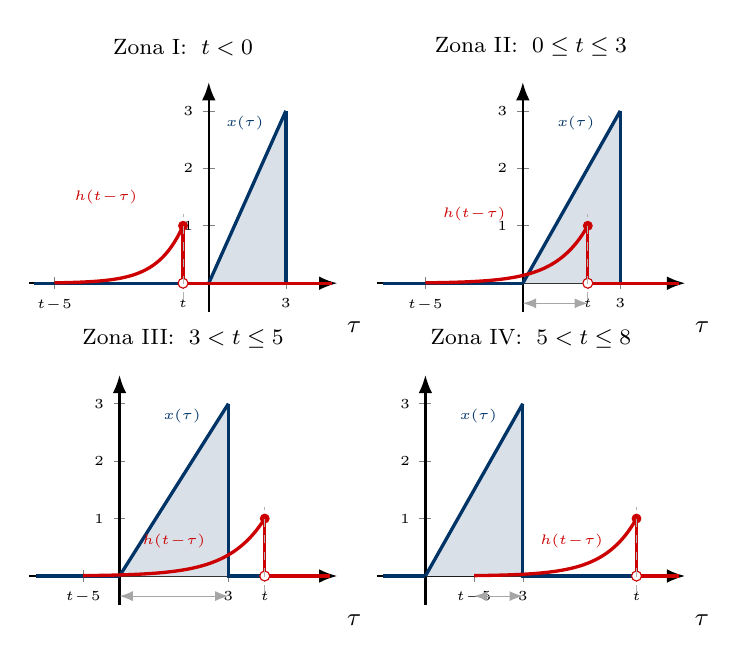
\begin{tikzpicture}[>=Latex, font=\small]

\colorlet{xcol}{utnblue}
\colorlet{hcol}{red!80!black}

% =====================================================================
% ZONA I: t = -1 (sin solapamiento)
% =====================================================================
\begin{axis}[
    name=z1,
    width=5.5cm, height=4.5cm,
    axis lines=center,
    xlabel={$\tau$},
    xlabel style={anchor=north west, at={(axis description cs:1,0)}},
    xmin=-7, xmax=5,
    ymin=-0.5, ymax=3.5,
    clip=true,
    axis line style={->, thick},
    xtick={-6,-1,0,3},
    xticklabels={$t\!-\!5$,$t$,$0$,$3$},
    ytick={0,1,2,3},
    every tick label/.style={font=\tiny},
    title={\footnotesize Zona~I:\; $t < 0$},
]
    % x(τ): rampa [0,3]
    \fill[xcol!15] (axis cs:0,0) -- (axis cs:3,3) -- (axis cs:3,0) -- cycle;
    \draw[xcol, very thick]
        (axis cs:-6.8,0) -- (axis cs:0,0);
    \addplot[xcol, very thick, domain=0:3, samples=2] {x};
    \draw[xcol, very thick] (axis cs:3,3) -- (axis cs:3,0) -- (axis cs:4.8,0);
    \node[xcol, font=\tiny, above left] at (axis cs:2.5,2.5) {$x(\tau)$};

    % h(t-τ) con t=-1: e^{-(−1−τ)}=e^{1+τ} en [-6,-1]
    \addplot[hcol, very thick, domain=-6:-1, samples=80] {exp(1+x)};
    \addplot[hcol, very thick, domain=-1:4.8, samples=2] {0};
    \draw[hcol, very thick] (axis cs:-1,0) -- (axis cs:-1,1);
    \fill[hcol]  (axis cs:-1,1) circle (1.8pt);
    \fill[white] (axis cs:-1,0) circle (1.8pt);
    \draw[hcol]  (axis cs:-1,0) circle (1.8pt);
    \node[hcol, font=\tiny] at (axis cs:-4,1.5) {$h(t\!-\!\tau)$};

    \draw[dashed, gray!60, thin] (axis cs:-1,-0.3) -- (axis cs:-1,1.2);
    \node[font=\tiny, gray, below] at (axis cs:1.5,-0.35) {$y(t)=0$};
\end{axis}

% =====================================================================
% ZONA II: t = 2 (solapamiento [0, t]=[0,2])
% =====================================================================
\begin{axis}[
    name=z2,
    at={(z1.east)}, anchor=west, xshift=0.5cm,
    width=5.5cm, height=4.5cm,
    axis lines=center,
    xlabel={$\tau$},
    xlabel style={anchor=north west, at={(axis description cs:1,0)}},
    xmin=-4.5, xmax=5,
    ymin=-0.5, ymax=3.5,
    clip=true,
    axis line style={->, thick},
    xtick={-3, 0, 2, 3},
    xticklabels={$t\!-\!5$, $0$, $t$, $3$},
    ytick={0,1,2,3},
    every tick label/.style={font=\tiny},
    title={\footnotesize Zona~II:\; $0 \leq t \leq 3$},
]
    % solapamiento [0,2]
    \fill[gray!25] (axis cs:0,0) -- (axis cs:2,0) -- (axis cs:2,2) -- cycle;

    % x(τ): rampa [0,3]
    \fill[xcol!15] (axis cs:0,0) -- (axis cs:3,3) -- (axis cs:3,0) -- cycle;
    \draw[xcol, very thick] (axis cs:-4.3,0) -- (axis cs:0,0);
    \addplot[xcol, very thick, domain=0:3, samples=2] {x};
    \draw[xcol, very thick] (axis cs:3,3) -- (axis cs:3,0) -- (axis cs:4.8,0);
    \node[xcol, font=\tiny, above left] at (axis cs:2.5,2.5) {$x(\tau)$};

    % h(t-τ) con t=2: e^{τ-2} en [-3,2]
    \addplot[hcol, very thick, domain=-3:2, samples=80] {exp(x-2)};
    \addplot[hcol, very thick, domain=2:4.8, samples=2] {0};
    \draw[hcol, very thick] (axis cs:2,0) -- (axis cs:2,1);
    \fill[hcol]  (axis cs:2,1) circle (1.8pt);
    \fill[white] (axis cs:2,0) circle (1.8pt);
    \draw[hcol]  (axis cs:2,0) circle (1.8pt);
    \node[hcol, font=\tiny] at (axis cs:-1.5,1.2) {$h(t\!-\!\tau)$};

    \draw[dashed, gray!60, thin] (axis cs:2,-0.3) -- (axis cs:2,1.2);
    \draw[<->, gray!70, thin] (axis cs:0,-0.35) -- (axis cs:2,-0.35);
    \node[font=\tiny, gray, below] at (axis cs:1,-0.35) {solap.};
\end{axis}

% =====================================================================
% ZONA III: t = 4 (solapamiento [0, 3]: x queda cubierto completo)
% =====================================================================
\begin{axis}[
    name=z3,
    at={(z1.south west)}, anchor=north west, yshift=-0.8cm,
    width=5.5cm, height=4.5cm,
    axis lines=center,
    xlabel={$\tau$},
    xlabel style={anchor=north west, at={(axis description cs:1,0)}},
    xmin=-2.5, xmax=6,
    ymin=-0.5, ymax=3.5,
    clip=true,
    axis line style={->, thick},
    xtick={-1, 0, 3, 4},
    xticklabels={$t\!-\!5$, $0$, $3$, $t$},
    ytick={0,1,2,3},
    every tick label/.style={font=\tiny},
    title={\footnotesize Zona~III:\; $3 < t \leq 5$},
]
    % solapamiento [0,3]: cubre todo x
    \fill[gray!25] (axis cs:0,0) -- (axis cs:3,3) -- (axis cs:3,0) -- cycle;

    % x(τ): rampa [0,3]
    \fill[xcol!15] (axis cs:0,0) -- (axis cs:3,3) -- (axis cs:3,0) -- cycle;
    \draw[xcol, very thick] (axis cs:-2.3,0) -- (axis cs:0,0);
    \addplot[xcol, very thick, domain=0:3, samples=2] {x};
    \draw[xcol, very thick] (axis cs:3,3) -- (axis cs:3,0) -- (axis cs:5.8,0);
    \node[xcol, font=\tiny, above left] at (axis cs:2.5,2.5) {$x(\tau)$};

    % h(t-τ) con t=4: e^{τ-4} en [-1,4]
    \addplot[hcol, very thick, domain=-1:4, samples=80] {exp(x-4)};
    \addplot[hcol, very thick, domain=4:5.8, samples=2] {0};
    \draw[hcol, very thick] (axis cs:4,0) -- (axis cs:4,1);
    \fill[hcol]  (axis cs:4,1) circle (1.8pt);
    \fill[white] (axis cs:4,0) circle (1.8pt);
    \draw[hcol]  (axis cs:4,0) circle (1.8pt);
    \node[hcol, font=\tiny] at (axis cs:1.5,0.6) {$h(t\!-\!\tau)$};

    \draw[dashed, gray!60, thin] (axis cs:4,-0.3) -- (axis cs:4,1.2);
    \draw[<->, gray!70, thin] (axis cs:0,-0.35) -- (axis cs:3,-0.35);
    \node[font=\tiny, gray, below] at (axis cs:1.5,-0.35) {solap.};
\end{axis}

% =====================================================================
% ZONA IV: t = 6.5 (solapamiento [t-5, 3]=[1.5, 3])
% =====================================================================
\begin{axis}[
    name=z4,
    at={(z3.east)}, anchor=west, xshift=0.5cm,
    width=5.5cm, height=4.5cm,
    axis lines=center,
    xlabel={$\tau$},
    xlabel style={anchor=north west, at={(axis description cs:1,0)}},
    xmin=-1.5, xmax=8,
    ymin=-0.5, ymax=3.5,
    clip=true,
    axis line style={->, thick},
    xtick={0, 1.5, 3, 6.5},
    xticklabels={$0$, $t\!-\!5$, $3$, $t$},
    ytick={0,1,2,3},
    every tick label/.style={font=\tiny},
    title={\footnotesize Zona~IV:\; $5 < t \leq 8$},
]
    % solapamiento [1.5, 3]
    \fill[gray!25] (axis cs:1.5,0) -- (axis cs:1.5,1.5) -- (axis cs:3,3) -- (axis cs:3,0) -- cycle;

    % x(τ): rampa [0,3]
    \fill[xcol!15] (axis cs:0,0) -- (axis cs:3,3) -- (axis cs:3,0) -- cycle;
    \draw[xcol, very thick] (axis cs:-1.3,0) -- (axis cs:0,0);
    \addplot[xcol, very thick, domain=0:3, samples=2] {x};
    \draw[xcol, very thick] (axis cs:3,3) -- (axis cs:3,0) -- (axis cs:7.8,0);
    \node[xcol, font=\tiny, above left] at (axis cs:2.5,2.5) {$x(\tau)$};

    % h(t-τ) con t=6.5: e^{τ-6.5} en [1.5,6.5]
    \addplot[hcol, very thick, domain=1.5:6.5, samples=80] {exp(x-6.5)};
    \addplot[hcol, very thick, domain=6.5:7.8, samples=2] {0};
    \draw[hcol, very thick] (axis cs:6.5,0) -- (axis cs:6.5,1);
    \fill[hcol]  (axis cs:6.5,1) circle (1.8pt);
    \fill[white] (axis cs:6.5,0) circle (1.8pt);
    \draw[hcol]  (axis cs:6.5,0) circle (1.8pt);
    \node[hcol, font=\tiny] at (axis cs:4.5,0.6) {$h(t\!-\!\tau)$};

    \draw[dashed, gray!60, thin] (axis cs:6.5,-0.3) -- (axis cs:6.5,1.2);
    \draw[<->, gray!70, thin] (axis cs:1.5,-0.35) -- (axis cs:3,-0.35);
    \node[font=\tiny, gray, below] at (axis cs:2.25,-0.35) {solap.};
\end{axis}

\end{tikzpicture}
\end{document}
